\section{Identiteit}

\textit{
  In dit hoofdstuk wordt de vraag ``Waaruit bestaat het onderdeel Identity Management binnen Blockchain technologie?'' behandeld. Zoals beschreven in hoofdstuk \ref{chapter:blockchain} zijn anonimiteit en controleerbaarheid belangrijke eigenschappen van een Blockchain implementatie. Allereerst zal er beschreven worden wat identiteit inhoud binnen een Blockchain en welke mogelijke vormen van management er zijn. Het antwoord op deze vraag wordt gebruikt om zoektermen op te stellen en een afbakening te creëren voor de te onderzoeken protocollen.
}

\begin{wrapfigure}[12]{r}{0.5\textwidth}
  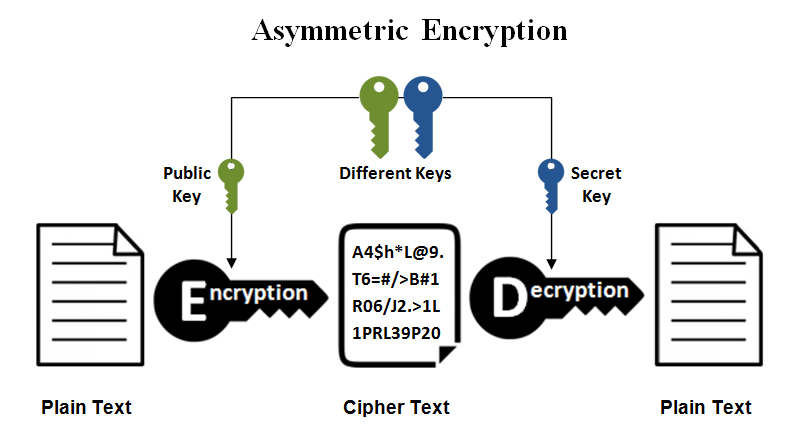
\includegraphics[width=0.5\textwidth]{figures/asymmetric_encryption}
  \caption[Asymmetrische encryptie]{
    Asymmetrische encryptie door middel van Public key cryptografie zoals in gebruik bij het Bitcoin protocol.
  }
  \label{asymmetric_encryption}    
\end{wrapfigure}

Identificatie wordt doorgaans gedaan aan de hand van de public key van een gebruiker. Public key cryptografie is een essentieel onderdeel van het Bitcoin protocol en wordt gebruikt voor verschillende doeleinden om de integriteit van berichten die verstuurd worden te waarborgen. Public key cryptografie bestaat uit twee onderdelen:

\begin{itemize}
  \item Public key
  \\ Een key die verstuurd wordt om aan te tonen dat een bericht daadwerkelijk verstuurd is door de maker van het bericht, door het ondertekenen van het bericht.
  \item Private key
  \\ Een key die geheim wordt gehouden en gebruikt wordt om te valideren dat een public key valide is.
\end{itemize}

\begin{wrapfigure}[6]{l}{0.3\textwidth}
  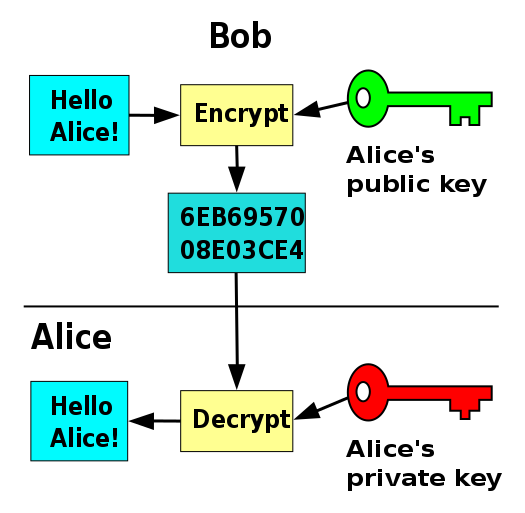
\includegraphics[width=0.3\textwidth]{figures/asymmetric_encryption_example}
  \caption[Gebruik van asymmetrische encryptie]{
    Het gebruik van asymmetrische encryptie om berichten die verstuurd worden op het netwerk te versleutelen.
  }
  \label{asymmetric_encryption_example}    
\end{wrapfigure}

In fig. \ref{asymmetric_encryption} is te zien hoe het gebruikt kan worden om tekst te versleutelen en alleen leesbaar te maken voor de ontvanger. Fig. \ref{asymmetric_encryption_example} laat zien hoe dit in zijn werk gaat met twee actoren. Bob stuurt een bericht naar Alice, waarbij de public key van Alice gebruikt wordt om het bericht te versleutelen. Om het bericht te kunnen lezen kan Alice gebruik maken van haar eigen private key. 

\newpage
In het Bitcoin protocol is elke coin terug te leiden naar een eigenaar waarbij er gebruik gemaakt wordt van de public key. Wanneer er coins van eigenaar wisselen worden de coins overgezet naar de public key van de ontvanger en wordt het getekend met de private key van de verstuurder. Dit zorgt ervoor dat iedereen in het netwerk weet dat het bericht authentiek is \citep[``How bitcoin works'']{bitcoin_wiki}.

\subsection{Autorisatie}

\cite{zheng2017overview} deelt Blockchain implementaties op in drie categorieën, waarin de zichtbaarheid en participatie in het consensus proces gelimiteerd.

\paragraph{Public} In een public Blockchain zijn alle transacties publiekelijk inzichtbaar en iedereen in het netwerk maakt onderdeel uit van het consensus proces. Dit wordt ook wel gezien als een permissionless Blockchain.

\paragraph{Consortium} In een consortium Blockchain is er een groep van vooraf geselecteerde nodes die deel uitmaken van het consensus proces. De consortium Blockchain wordt meestal gebruikt door meerdere organisaties en is gedeeltelijk gedecentraliseerd. Omdat bepaalde nodes geïdentificeerd dienen te worden wordt dit type Blockchain gezien als een permissioned Blockchain.

\paragraph{Private} In een private Blockchain worden alleen nodes van een specifieke organisatie toegelaten tot het consensus proces. Het wordt ook wel als een centraal netwerk gezien omdat het in volledige controle is van één organisatie. Omdat het hier gaat om volledige restrictie tot het Blockchain netwerk wordt dit type Blockchain gezien als een permissioned Blockchain.

In een consortium en private Blockchain dient de gebruiker zich te identificeren aan de hand van een identiteit. Bitcoin maakt gebruik van public- en private keys om de gebruiker te identificeren. Dit hanteert in zekere mate een permissie model waarbij de autorisatie van een gebruiker vastgelegd word aan de hand van de identificatie (i.e.\ de public key) die het netwerk gebruikt.

\subsubsection{Privacy}

Een van de doelen van Blockchain is totale anonimiteit, alleen zijn er een aantal problemen die volledige anonimiteit tegengaan. Om de terminologie duidelijk te maken wordt hieronder het verschil tussen pseudoniem en anoniem uitgelegd aan de hand van voorbeelden vanuit het Bitcoin protocol.

\begin{formal}
  ``Anonymity is the state of being not identifiable within a set of subjects, the anonymity set."
  \\ \cite{pfitzmann2001anonymity}.
\end{formal}

\paragraph{Pseudoniem} 

Een pseudoniem is een referentie naar je ware identiteit. Een voorbeeld hiervan is het burgerservicenummer (BSN). Door het geven van je BSN is niet direct je ware identiteit terug te leiden.

\paragraph{Anoniem}

Wanneer je anoniem bent, ben je niet meer te identificeren binnen een set van soortgelijke identiteiten. Een voorbeeld hiervan is anoniem bellen. Hierbij wordt er gebruik gemaakt van het maskeren van het pseudoniem, namelijk het telefoonnummer.

In feite komt het neer op de identificatie van de handelingen die gedaan worden door de gebruiker. Hiervoor bestaat een term, unlinkability, dat beschrijft wanneer een gebruiker meerdere keren interacteert met het systeem deze handelingen niet terug te leiden zijn naar elkaar.

\subsubsection{Privacy in Bitcoin}

In Bitcoin is de identiteit van de gebruiker, de public key(s), een pseudoniem. Aangezien Bitcoin een permissionless model heeft, waarbij iedereen elke transactie kan inzien, is het mogelijk om transacties die gedaan zijn door dezelfde public key terug te leiden naar elkaar.

Een analyse model geïntroduceerd door \cite{reid2013analysis} maakt gebruik van twee modellen van het Bitcoin netwerk, waarbij er een model gemaakt wordt voor bitcoins tussen transacties, en bitcoins tussen gebruikers. Door het gebruik van de voortgestelde analyse is het mogelijk om meerdere public keys met elkaar te associëren. 

